\documentclass[12pt,addpoints]{repaso}
\grado{2}
\nivel{Secundaria}
\cicloescolar{2024-2025}
\materia{Matemáticas}
\unidad{1}
\title{Repaso para el examen de la Unidad}
\aprendizajes{
        \item Resuelve problemas de multiplicación y división con números enteros, fracciones y decimales positivos y negativos.
        \item Resuelve problemas de potencias con exponente entero y aproxima raíces cuadradas.
        \item Resuelve problemas de proporcionalidad directa e inversa y de reparto proporcional.
}
\author{Melchor Pinto, J.C.}
\begin{document}
\INFO%
\begin{questions}
      \questionboxed[10]{Escribe sobre la línea el símbolo de mayor que ($>$), menor que ($<$), o igual ($=$) según corresponda.

            \begin{multicols}{2}
                  \begin{parts}
                        \part $\dfrac{2}{5}$ \fillin[$>$][0.5in] $\dfrac{1}{3}$\\[0.25em]
                        \part $\dfrac{3}{4}$ \fillin[$<$][0.5in] $\dfrac{4}{5}$\\[0.25em]
                        \part $\dfrac{2}{5}$ \fillin[$<$][0.5in] $\dfrac{2}{3}$\\[0.25em]
                        \part $\dfrac{3}{2}$ \fillin[$=$][0.5in] $\dfrac{9}{6}$\\[0.25em]
                        \part $\dfrac{5}{6}$ \fillin[$>$][0.5in] $\dfrac{4}{6}$\\[0.25em]
                        \part $\dfrac{4}{3}$ \fillin[$>$][0.5in] $\dfrac{5}{4}$\\[0.25em]
                        \part $\dfrac{1}{3}$ \fillin[$=$][0.5in] $\dfrac{9}{3}$\\[0.25em]
                        \part $\dfrac{2}{3}$ \fillin[$<$][0.5in] $\dfrac{3}{2}$\\[0.25em]
                        \part $\dfrac{3}{4}$ \fillin[$>$][0.5in] $\dfrac{2}{3}$\\[0.25em]
                        \part $\dfrac{5}{6}$ \fillin[$>$][0.5in] $\dfrac{4}{5}$\\[0.25em]
                        \part $-51$ \fillin[$>$][0.5in] $-55$\\[0.25em]
                        \part $-77$ \fillin[$>$][0.5in] $-177$\\[0.25em]
                        \part $-100$ \fillin[$<$][0.5in] $-99$\\[0.25em]
                        \part $-182$ \fillin[$>$][0.5in] $-189$\\[0.25em]
                        \part $-97$ \fillin[$<$][0.5in] $-96.2$\\[0.25em]
                        \part $-36$ \fillin[$>$][0.5in] $-39$\\[0.25em]
                        \part $-3.5$ \fillin[$<$][0.5in] $-2.2$\\[0.25em]
                        \part $-12$ \fillin[$<$][0.5in] $-11$\\[0.25em]
                        \part $-10.001$ \fillin[$>$][0.5in] $-100.01$\\[0.25em]
                        \part $-0.99$ \fillin[$>$][0.5in] $1.01$
                  \end{parts}
            \end{multicols}
      }

      \newpage

      \questionboxed[20]{Realiza las operaciones con exponentes indicadas en cada uno de los siguientes incisos.

            \begin{multicols}{2}
                  \begin{parts}
                        \part $\dfrac{x^{13}y^{18}z^4}{x^{11}y^9z^4}=$
                        \begin{solutionbox}{2cm}
                              $\dfrac{x^{13}y^{18}z^4}{x^{11}y^9z^4} = x^2y^9$
                        \end{solutionbox}


                        \part $(-3a^4)(8a^2)=$
                        \begin{solutionbox}{2cm}
                              $(-3a^4)(8a^2) = -24a^6$
                        \end{solutionbox}

                        \part $4x^2\cdot x^5\cdot 5x^8=$
                        \begin{solutionbox}{2cm}
                              $4x^2\cdot x^5\cdot 5x^8 = 20x^{15}$
                        \end{solutionbox}



                        \part $\dfrac{81a^5b^{12}c^9}{9a^3b^{7}c^5}=$
                        \begin{solutionbox}{2cm}
                              $\dfrac{81a^5b^{12}c^9}{9a^3b^{7}c^5} = 9a^2b^5c^4$
                        \end{solutionbox}

                        \part $\dfrac{x^{4}y^{12}z^{13}}{x^{3}y^{12}z^{13}}=$
                        \begin{solutionbox}{2cm}
                              $\dfrac{x^{4}y^{12}z^{13}}{x^{3}y^{12}z^{13}} = x$
                        \end{solutionbox}

                        \part $\left(a^3 b^5 c^{11} \right)^7=$
                        \begin{solutionbox}{2cm}
                              $\left(a^3 b^5 c^{11} \right)^7 = a^{21}b^{35}c^{77}$
                        \end{solutionbox}

                        % \part  $x^3\cdot x^5\cdot x=$
                        % \begin{solutionbox}{2cm}
                        %       $x^3\cdot x^5\cdot x = x^9$
                        % \end{solutionbox}


                        % \part $\left(a^4b^4c^5d^{11}\right)^9=$
                        % \begin{solutionbox}{2cm}
                        %       $\left(a^4b^4c^5d^{11}\right)^9 = a^{36}b^{36}c^{45}d^{99}$
                        % \end{solutionbox}
                        \part $x^2y^3z^4 \cdot x^5z^4=$
                        \begin{solutionbox}{2cm}
                              $x^2y^3z^4 \cdot x^5z^4 = x^7y^3z^8$
                        \end{solutionbox}

                        \part $\left(x^4 y^5\right)^6=$
                        \begin{solutionbox}{2cm}
                              $\left(x^4 y^5\right)^6 = x^{24}y^{30}$
                        \end{solutionbox}

                        \part $x^3x^2x^3=$
                        \begin{solutionbox}{2cm}
                              $x^3x^2x^3 = x^8$
                        \end{solutionbox}

                        \part $7x^2\cdot 3x^4 \cdot 6x^2=$
                        \begin{solutionbox}{2cm}
                              $7x^2\cdot 3x^4 \cdot 6x^2 = 126x^8$
                        \end{solutionbox}
                        % \part $x^3x^2x^3=$
                        % \begin{solutionbox}{2cm}
                        %       $x^3x^2x^3 = x^8$
                        % \end{solutionbox}

                        % \part $7x^2\cdot 3x^4 \cdot 6x^2=$
                        % \begin{solutionbox}{2cm}
                        %       $7x^2\cdot 3x^4 \cdot 6x^2 = 126x^8$
                        % \end{solutionbox}

                        % \part $(-4x^2)(-5x^3)=$
                        % \begin{solutionbox}{2cm}
                        %       $(-4x^2)(-5x^3) = 20x^5$
                        % \end{solutionbox}

                        % \part $(-8x)(-5x^5)=$
                        % \begin{solutionbox}{2cm}
                        %       $(-8x)(-5x^5) = 40x^6$
                        % \end{solutionbox}

                        % \part $(-x^4)(2y^3)=$
                        % \begin{solutionbox}{2cm}
                        %       $(-x^4)(2y^3) = -2x^4y^3$
                        % \end{solutionbox}

                        % \part $(-5a^4)(-3a^2)=$
                        % \begin{solutionbox}{2cm}
                        %       $(-5a^4)(-3a^2) = 15a^6$
                        % \end{solutionbox}
                  \end{parts}
            \end{multicols}
      }

      \questionboxed[10]{Realiza las operaciones con exponentes indicadas en cada uno de los siguientes incisos.

            % \begin{multicols}{2}
            \begin{parts}
                  % \part $x^2y^3z^4 \cdot x^5z^4=$
                  % \begin{solutionbox}{2cm}
                  %       $x^2y^3z^4 \cdot x^5z^4 = x^7y^3z^8$
                  % \end{solutionbox}



                  \part $(-4x^2)(-5x^3)=$
                  \begin{solutionbox}{2cm}
                        $(-4x^2)(-5x^3) = 20x^5$
                  \end{solutionbox}

                  \part $(-8x)(-5x^5)=$
                  \begin{solutionbox}{2cm}
                        $(-8x)(-5x^5) = 40x^6$
                  \end{solutionbox}

                  \part $(-x^4)(2y^3)=$
                  \begin{solutionbox}{2cm}
                        $(-x^4)(2y^3) = -2x^4y^3$
                  \end{solutionbox}

                  \part $(-5a^4)(-3a^2)=$
                  \begin{solutionbox}{2cm}
                        $(-5a^4)(-3a^2) = 15a^6$
                  \end{solutionbox}

                  \part  $x^3\cdot x^5\cdot x=$
                  \begin{solutionbox}{2cm}
                        $x^3\cdot x^5\cdot x = x^9$
                  \end{solutionbox}

                  % \part $(-3a^4)(8a^2)=$
                  % \begin{solutionbox}{2cm}
                  %       $(-3a^4)(8a^2) = -24a^6$
                  % \end{solutionbox}

                  % \part $4x^2\cdot x^5\cdot 5x^8=$
                  % \begin{solutionbox}{2cm}
                  %       $4x^2\cdot x^5\cdot 5x^8 = 20x^{15}$
                  % \end{solutionbox}

                  % \part $\dfrac{x^{13}y^{18}z^4}{x^{11}y^9z^4}=$
                  % \begin{solutionbox}{2cm}
                  %       $\dfrac{x^{13}y^{18}z^4}{x^{11}y^9z^4} = x^2y^9$
                  % \end{solutionbox}

                  % \part $\dfrac{81a^5b^{12}c^9}{9a^3b^{7}c^5}=$
                  % \begin{solutionbox}{2cm}
                  %       $\dfrac{81a^5b^{12}c^9}{9a^3b^{7}c^5} = 9a^2b^5c^4$
                  % \end{solutionbox}

                  % \part $\dfrac{x^{4}y^{12}z^{13}}{x^{3}y^{12}z^{13}}=$
                  % \begin{solutionbox}{2cm}
                  %       $\dfrac{x^{4}y^{12}z^{13}}{x^{3}y^{12}z^{13}} = x$
                  % \end{solutionbox}

                  % \part $\left(a^3 b^5 c^{11} \right)^7=$
                  % \begin{solutionbox}{2cm}
                  %       $\left(a^3 b^5 c^{11} \right)^7 = a^{21}b^{35}c^{77}$
                  % \end{solutionbox}

                  % \part $\left(x^4 y^5\right)^6=$
                  % \begin{solutionbox}{2cm}
                  %       $\left(x^4 y^5\right)^6 = x^{24}y^{30}$
                  % \end{solutionbox}

                  % \part $\left(a^4b^4c^5d^{11}\right)^9=$
                  % \begin{solutionbox}{2cm}
                  %       $\left(a^4b^4c^5d^{11}\right)^9 = a^{36}b^{36}c^{45}d^{99}$
                  % \end{solutionbox}

            \end{parts}
            % \end{multicols}
      }

      \newpage
      \questionboxed[10]{Escribe el número que representa el punto indicado en la recta numérica de cada uno de los siguientes incisos.

            \begin{multicols}{2}
                  \begin{parts}
                        \part 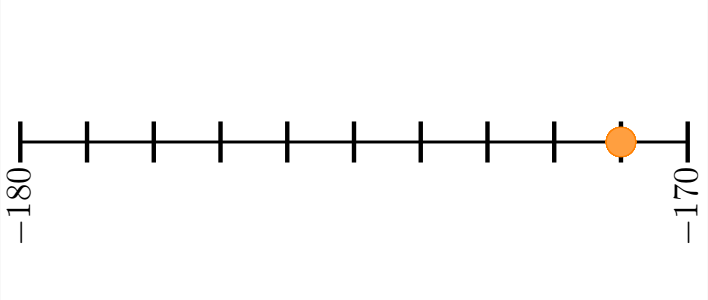
\includegraphics[width=140px]{../images/recta_num_-171.png} \\[-0.5em]   \fillin[$-171$][1.5in]
                        \part 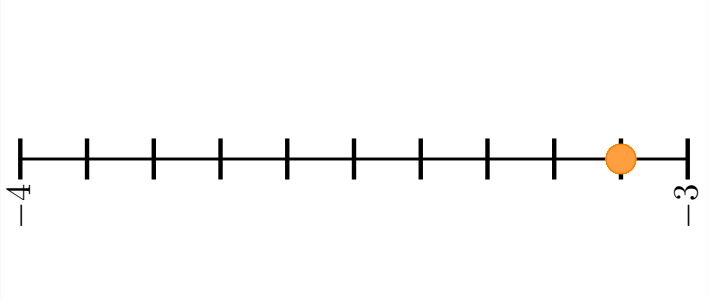
\includegraphics[width=140px]{../images/recta_num_-3.1.png} \\[-0.5em]   \fillin[$-3.1$][1.5in]
                        \part 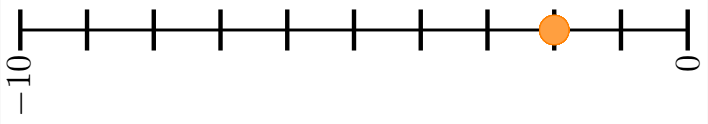
\includegraphics[width=140px]{../images/recta_num_-2.png}   \\[-0.5em] \fillin[$-2$][1.5in]
                        \part 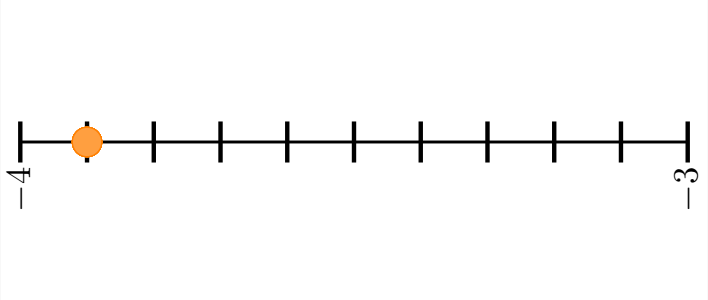
\includegraphics[width=140px]{../images/recta_num_-3.9.png} \\[-0.5em]   \fillin[$-3.9$][1.5in]
                        \part 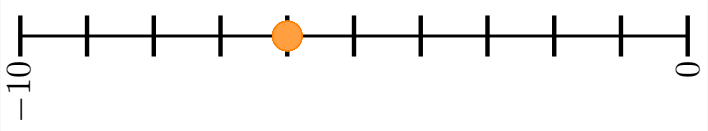
\includegraphics[width=140px]{../images/recta_num_-6.png}   \\[-0.5em] \fillin[$-6$][1.5in]
                        \part 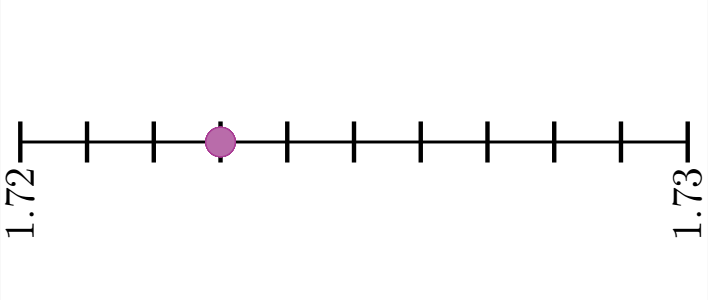
\includegraphics[width=140px]{../images/recta_num_1.723.png}\\[-0.5em]  \fillin[$1.723$][1.5in]
                        \part 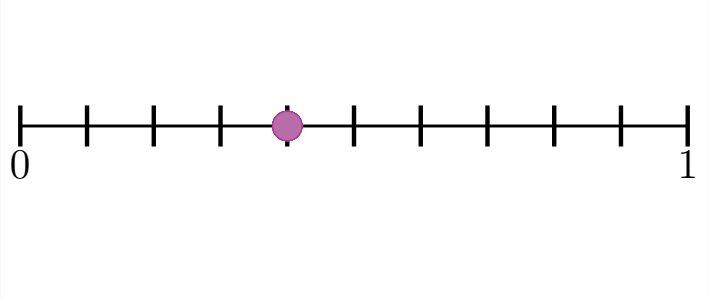
\includegraphics[width=140px]{../images/recta_num_0.4.png}  \\[-0.5em]  \fillin[$0.4.$][1.5in]
                        \part 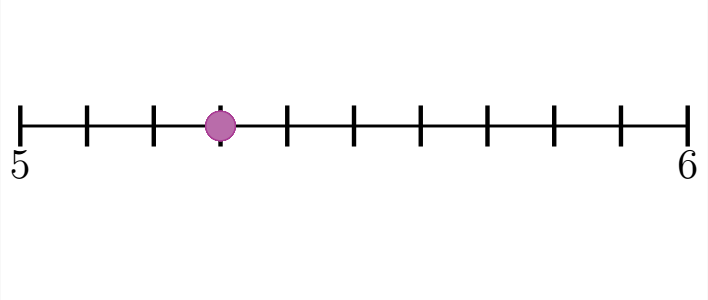
\includegraphics[width=140px]{../images/recta_num_5.3.png}  \\[-0.5em]  \fillin[$5.3.$][1.5in]
                        \part 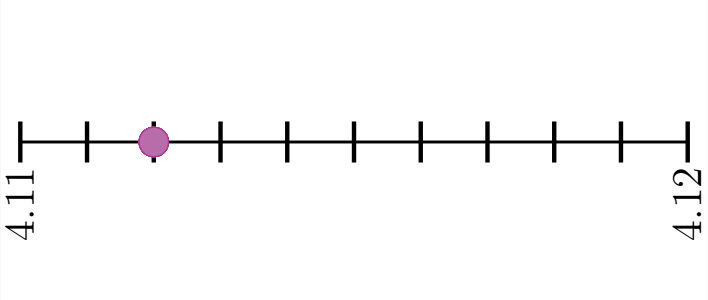
\includegraphics[width=140px]{../images/recta_num_4.112.png}\\[-0.5em]  \fillin[$4.11$][1.5in]
                        \part 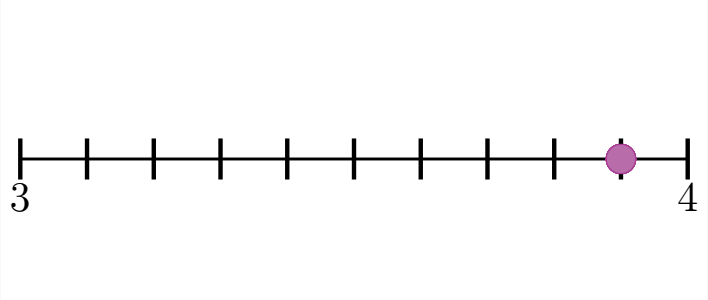
\includegraphics[width=140px]{../images/recta_num_3.9.png}  \\[-0.5em]  \fillin[$3.9.$][1.5in]
                  \end{parts}
            \end{multicols}
      }

      \questionboxed[10]{Convierte los siguientes números en notación decimal a notación científica en la forma más reducida posible.
            \begin{multicols}{2}
                  \begin{parts}
                        \part $50500=$ \fillin[$5.05 \cdot 10^4$][1.5in]
                        \part $0.00000000024=$ \fillin[$2.4 \cdot 10^{-10}$][1.5in]
                        \part $101=$ \fillin[$1.01 \cdot 10^2$][1.5in]
                        \part $750000000000=$ \fillin[$7.5 \cdot 10^{11}$][1.5in]
                        \part $80008000=$ \fillin[$8.0008 \cdot 10^7$][1.5in]
                        \part $0.003=$ \fillin[$3 \cdot 10^{-3}$][1.5in]
                        \part $0.0000204=$ \fillin[$2.04 \cdot 10^{-5}$][1.5in]
                        \part $0.0000000000099=$ \fillin[$9.9 \cdot 10^{-12}$][1.5in]
                        \part $606000000000000000=$ \fillin[$6.06 \cdot 10^{17}$][1.5in]
                        \part $102100000000000=$ \fillin[$1.001 \cdot 10^{-7}$][1.5in]
                  \end{parts}
            \end{multicols}
      }

      \questionboxed[10]{Escribe el número que representa el punto indicado en la recta numérica de cada uno de los siguientes incisos.

            \begin{multicols}{2}
                  \begin{parts}
                        \part 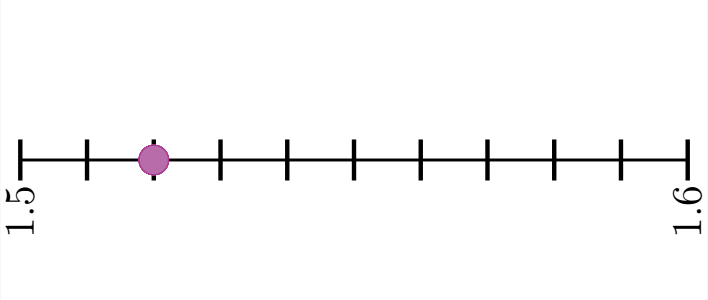
\includegraphics[width=150px]{../images/recta_num_1.52.png} \\[-0.5em] \fillin[$1.52$][1.5in]   \\[-1.4em]
                        \part 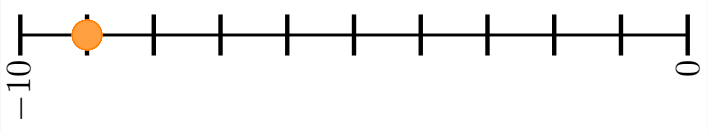
\includegraphics[width=150px]{../images/recta_num_-9.png}   \\[-0.5em] \fillin[$-9$][1.5in]     \\[-1.4em]
                        \part 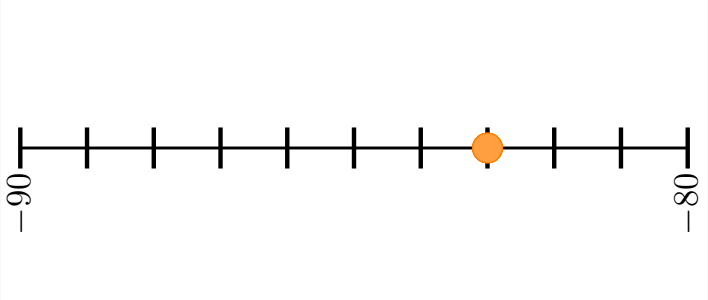
\includegraphics[width=150px]{../images/recta_num_-83.png}  \\[-0.5em]  \fillin[$-83$][1.5in]   \\[-1.4em]
                        \part 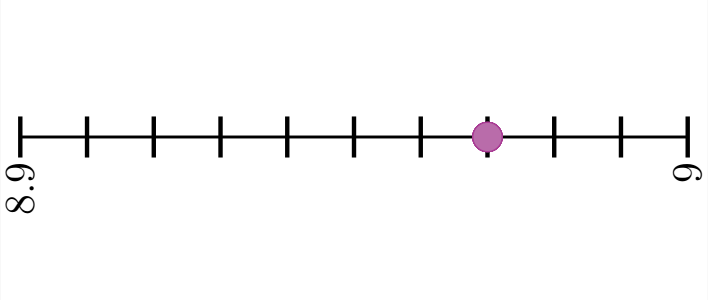
\includegraphics[width=150px]{../images/recta_num_8.97.png} \\[-0.5em]  \fillin[$8.97$][1.5in]  \\[-1.4em]
                        \part 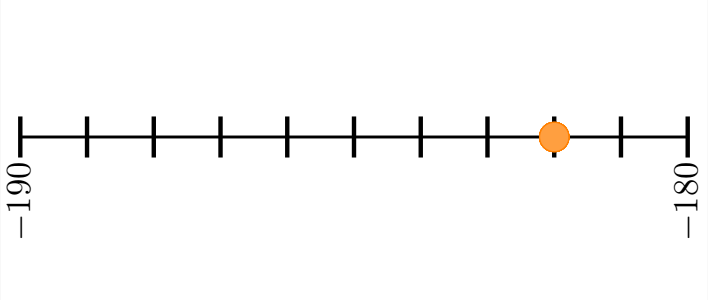
\includegraphics[width=150px]{../images/recta_num_-182.png} \\[-0.5em]   \fillin[$-182$][1.5in] \\[-1.4em]
                        \part 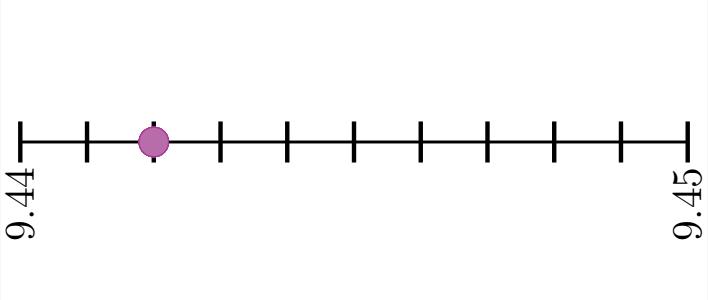
\includegraphics[width=150px]{../images/recta_num_9.442.png}\\[-0.5em]  \fillin[$9.44$][1.5in]  \\[-1.4em]
                        \part 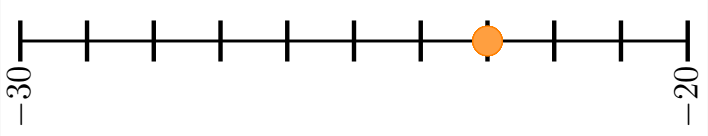
\includegraphics[width=150px]{../images/recta_num_-23.png}  \\[-0.5em]  \fillin[$-23$][1.5in]   \\[-1.4em]
                        \part 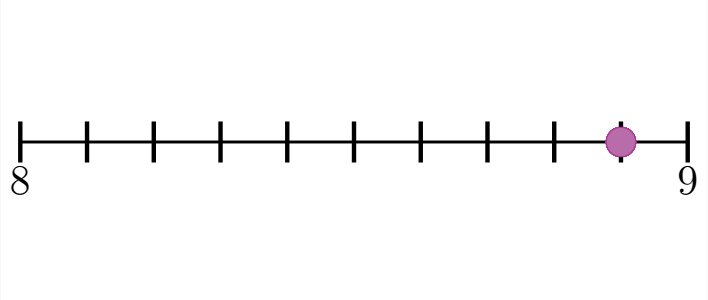
\includegraphics[width=150px]{../images/recta_num_8.9.png}  \\[-0.5em]  \fillin[$8.9$][1.5in]   \\[-1.4em]
                        \part 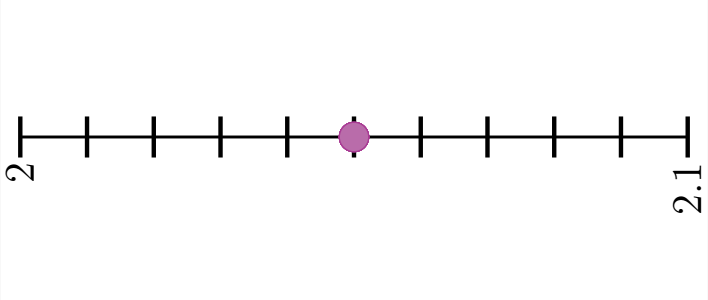
\includegraphics[width=150px]{../images/recta_num_2.05.png} \\[-0.5em]  \fillin[$2.05$][1.5in]  \\[-1.4em]
                        \part 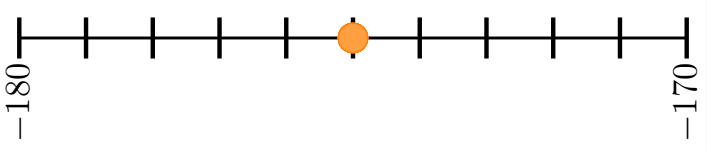
\includegraphics[width=150px]{../images/recta_num_-175.png} \\[-0.5em]   \fillin[$-175$][1.5in]
                  \end{parts}
            \end{multicols}
      }
      \questionboxed[10]{Convierte los siguientes números en notación científica a notación decimal.
            \begin{multicols}{2}
                  \begin{parts}
                        \part $1.2 \cdot 10^3=$ \fillin[$1200$][1.5in]
                        \part $2.3 \cdot 10^2=$ \fillin[$230$][1.5in]
                        \part $4 \cdot 10^{-3}=$ \fillin[$0.004$][1.5in]
                        \part $7 \cdot 10^{-6}=$ \fillin[$0.000007$][1.5in]
                        \part $2 \cdot 10^6=$ \fillin[$2000000$][1.5in]
                        \part $-3 \cdot 10^{-4}=$ \fillin[$-0.0003$][1.5in]
                        \part $1.2 \cdot 10^{-1}=$ \fillin[$0.12$][1.5in]
                        \part $80.3 \cdot 10^{-2}=$ \fillin[$0.803$][1.5in]
                        \part $3 \cdot 10^{-3}=$ \fillin[$0.003$][1.5in]
                        \part $3 \cdot 10^{8}=$ \fillin[$300000000$][1.5in]
                  \end{parts}
            \end{multicols}
      }
\end{questions}
\end{document}